\subsection{Normalized Step Length
  (\robustInlinecode{Alpha})}\label{cockpit::app:alpha}

\begin{figure*}
  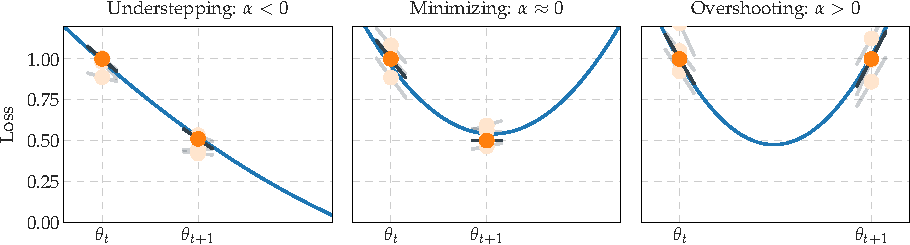
\includegraphics[width =
  \linewidth]{../repos/cockpit-paper/fig/12_alpha_explanation/output/alpha_explanation_thesis-wide}
  \caption{\textbf{Motivational sketch for the $\alpha$ quantity.} In each
    iteration of the optimizer we observe the loss function at two positions
    $\vtheta_{t}$ and $\vtheta_{t+1}$ (shown in
    \textcolor{sns_orange}{\ding{108}}). The black lines
    (\textcolor{TUdark}{\textbf{---}}) show the observed slope at this position,
    which we can get from projecting the gradients onto the current step
    direction $\vtheta_{t+1} - \vtheta_{t}$. Note, that all four observations
    (two loss and two slope values) are noisy, due to being computed on a
    mini-batch. With access to the individual losses and gradients (some samples
    shown in
    \textcolor{sns_orange_light}{\ding{108}}/\textcolor{TUgray}{\textbf{---}}),
    we can estimate their noise level and build a noise-informed quadratic fit
    (\textcolor{sns_blue}{\textbf{---}}). Using this fit, we determine whether
    the optimizer minimizes the local uni-variate loss (\textit{middle plot}), or
    whether we understep (\textit{left plot}) or overshoot (\textit{right plot})
    the minimum.}
  \label{cockpit::fig:alpha_explanation}
\end{figure*}

\subsubsection{Motivation}

The goal of the $\alpha$-quantity is to estimate and quantify the effect that a
selected learning rate has on the optimizer's steps. Consider the optimizer's
step at training iteration $t$. This parameter update from $\vtheta_{t}$ to
$\vtheta_{t+1}$ happens in a one-dimensional space, defined by the update
direction $\vtheta_{t+1} - \vtheta_{t}=\vs_t$. The update direction depends on
the update rule of the optimizer, \eg for \sgd with learning rate $\eta$ it is
simply $\vs_t =- \eta \vg_{\sB_t}(\vtheta_{t})$.

We build a noise-informed uni-variate quadratic approximation along this update
step ($\vtheta_{t} \to \vtheta_{t+1}$) based on the two noisy loss function
observations at $\vtheta_{t}$ and $\vtheta_{t+1}$ and the two noisy slope
observation at these two points. Examining this quadratic fit, we are able to
determine where on this parabola our optimizer steps. Standardizing this, we
express a step to the minimum of the loss in the update direction as $\alpha=0$.
Analogously, steps that end short of this minimum result in $\alpha<0$, and a
step over the minimum in $\alpha>0$. These three different scenarios are
illustrated in \Cref{cockpit::fig:alpha_explanation} also showing the underlying
observations that would lead to them. \Cref{cockpit::fig:LINE} shows the distribution of
$\alpha$-values for two very different optimization trajectories.

\subsubsection{Noisy Observations}

In order to build an approximation for the loss function in the update
direction, we leverage the four observations of the function (and its
derivative) that are available in each iteration. Due to the stochasticity of
deep learning optimization, we also take into account the noise-level of all
observations by estimating them. The first two observations are the mini-batch
training losses $\mathcal{L}_{\sB_t}(\vtheta_t),
\mathcal{L}_{\sB_{t+1}}(\vtheta_{t+1})$ at point $\vtheta_{t}$ and
$\vtheta_{t+1}$, which are computed in every standard training loop. The
mini-batch losses are averages over individual losses,
\begin{align*}
  \mathcal{L}_{\sB_t}(\vtheta_t)
  &=
    \E_{\sB_t}\left[ \ell(\vtheta_t) \right] = \frac{1}{|\sB_t|} \sum_{n \in \sB_t}
    \ell_n(\vtheta_t) \,,
  \\
  \mathcal{L}_{\sB_{t+1}}(\vtheta_{t+1})
  &=
    \E_{\sB_{t+1}}\left[ \ell(\vtheta_{t+1}) \right] = \frac{1}{|\sB_{t+1}|} \sum_{n \in \sB_{t+1}}
    \ell_n(\vtheta_{t+1})\,,
\end{align*}
and using these individual losses, we can also compute the variances to estimate
the noise-level of our loss observation,
\begin{align*}
  \Var_{\sB_{t}} \left[ \ell(\vtheta_t) \right]
  =&
     \left( \frac{1}{|\sB_t|} \sum_{n \in \sB_t} \ell_n(\vtheta_t)^2 \right)
     -
     \left( \frac{1}{|\sB_t|} \sum_{n \in \sB_t} \ell_n(\vtheta_t) \right)^2 \, ,
  \\
  \Var_{\sB_{t+1}} \left[ \ell(\vtheta_{t+1}) \right]
  =&
     \left( \frac{1}{|\sB_{t+1}|} \sum_{n \in \sB_{t+1}} \ell_n(\vtheta_{t+1})^2 \right)
     -
     \left( \frac{1}{|\sB_{t+1}|} \sum_{n \in \sB_{t+1}} \ell_n(\vtheta_{t+1}) \right)^2 \, .
\end{align*}
Similarly, we proceed with the slope in the update direction. To compute the
slope of the loss function in the direction of the optimizer's update $\vs_t$,
we project the current gradient along this update direction
\begin{align*}
  \E_{\sB_t} \left[\frac{\vs_t^\top \vg(\vtheta_t)}{\lVert \vs_t
  \rVert^2}\right]
  =&
     \frac{1}{|\sB_{t}|} \sum_{n\in \sB_t} \frac{\vs_t^\top \vg_n(\vtheta_t)}{\lVert
     \vs_t \rVert^2} \, ,
  \\
  \E_{\sB_{t+1}} \left[\frac{\vs_t^\top \vg(\vtheta_{t+1})}{\lVert \vs_t
  \rVert^2}\right]
  =&
     \frac{1}{|\sB_{t+1}|} \sum_{n\in \sB_{t+1}} \frac{\vs_t^\top \vg_n(\vtheta_{t+1})}{\lVert
     \vs_t \rVert^2} \, .
\end{align*}
Just like before, we can also compute the variance of this slope, by leveraging
individual gradients,
\begin{align*}
  &\Var_{\sB_t} \left[\frac{\vs_t^\top \vg(\vtheta_t)}{\lVert \vs_t
  \rVert^2}\right]
    \\
  &\quad=
     \frac{1}{|\sB_t|} \sum_{n\in B_t} \left( \frac{\vs_t^\top \vg_n(\vtheta_t)}{\lVert
     \vs_t \rVert^2} \right)^2
     -  \left( \frac{1}{|\sB_t|} \sum_{n\in \sB_t} \frac{\vs_t^\top
     \vg_n(\vtheta_t)}{\lVert \vs_t \rVert^2} \right)^2 \, ,
  \\
  &\Var_{\sB_{t+1}} \left[\frac{\vs_t^\top \vg(\vtheta_{t+1})}{\lVert \vs_t
  \rVert^2}\right]
    \\
  &\quad=
     \frac{1}{|\sB_{t+1}|} \sum_{n\in \sB_{t+1}} \left( \frac{\vs_t^\top \vg_n(\vtheta_{t+1})}{\lVert
     \vs_t \rVert^2} \right)^2
     -  \left( \frac{1}{|\sB_{t+1}|} \sum_{n\in \sB_{t+1}} \frac{\vs_t^\top
     \vg_n(\vtheta_{t+1})}{\lVert \vs_t \rVert^2} \right)^2 \, .
\end{align*}

\subsubsection{Quadratic Fit \& Normalization}

Using our (noisy) observations, we are now ready to build an approximation for
the loss as a function of the step size, which we will denote as $f(\tau)$. We
assume a quadratic function for $f$, which follows recent reports for the loss
landscape of neural networks \citep{xing2018walk}, \ie a function $f(\tau) = w_0
+ w_1 \tau + w_2 \tau^2$ parameterized by $\vw \in \R^3$. We further assume a
Gaussian likelihood of the form
\begin{align}
  \label{cockpit::eq:alpha_likelihood}
  p\left(\giventhat{\tilde{\vf}}{\vw, \mPhi}\right)
  =
  \mathcal{N}\left(\giventhat{\tilde{\vf}}{ \mPhi^\top \vw, \mLambda}\right)
\end{align}
for observations $\tilde{\vf}$ of the loss and its slope. The observation matrix
$\mPhi$ and the noise matrix of the observations $\mLambda$ are
\begin{align*}
  \mPhi = \begin{pmatrix}
    1 & 1 & 0 & 0 \\
    \tau_1 & \tau_2  & 1 & 1 \\
    \tau_1^2 & \tau_2^2 & 2\tau_1 &  2\tau_2
  \end{pmatrix}\,,
                                    \qquad \qquad
                                    \mLambda = \begin{pmatrix}
                                      \sigma_{\tilde{f}_1} & 0 & 0 & 0 \\ 0 & \sigma_{\tilde{f}_2} & 0 & 0  \\ 0
                                      & 0 & \sigma_{\tilde{f}'_1} & 0 \\ 0 & 0 & 0 & \sigma_{\tilde{f}'_2}
                                    \end{pmatrix} \, ,
\end{align*}
where $\tau$ denotes the position and $\sigma$ denotes the noise-level estimate
of the observation. The maximum likelihood solution of
\Cref{cockpit::eq:alpha_likelihood} for the parameters of our quadratic fit is given by
\begin{align}
  \label{cockpit::eq:alpha-feature-table}
  \vw = \left(\mPhi \mLambda^{-1}\mPhi^\top\right)^{-1}\mPhi \mLambda^{-1}
  \tilde{\vf} \, .
\end{align}
Once we have the quadratic fit of the uni-variate loss along the update
direction, we normalize the scales such that the resulting $\alpha$ expresses
the effective step taken by the optimizer sketched in
\Cref{cockpit::fig:alpha_explanation}.

\subsubsection{Usage}

The $\alpha$-quantity is related to recent line search approaches
\cite{mahsereci2017probabilistic,vaswani2019painless}. However, instead of searching for an
acceptable step by repeated attempts, we instead report the effect of the
current step size selection. This could, for example, be used to disentangle the
two optimization runs in \Cref{cockpit::fig:LINE}. Additionally, this information could
also be used to automatically adapt the learning rate during the training
process. But, as discussed in \Cref{cockpit::sec:alpha_exp}, it isn't trivial what the
``correct'' decision is, as it might depend on the optimization problem, the
training phase, and other factors. Having this $\alpha$-quantity can, however,
provide more insight into what kind of steps are used in well-tuned runs with
traditional optimizers such as \sgd.

%%% Local Variables:
%%% mode: latex
%%% TeX-master: "../thesis"
%%% End:
